\documentclass[portrait,a0]{a0poster}
\usepackage{color,multicol}
\usepackage[english]{babel}
\usepackage[utf8]{inputenc}
\usepackage[T1]{fontenc}
\usepackage{siunitx}
\usepackage{graphicx}
\usepackage{booktabs}
%\usepackage[round]{natbib}
\usepackage[font=small]{caption}
\usepackage{lmodern}
\usepackage[overload]{textcase}
\usepackage{setspace}
\usepackage{float}
\usepackage{titlesec}
\usepackage{lipsum} % Lorem ipsum generator
\usepackage{caption}
\usepackage{tikz}
\usetikzlibrary{shapes.arrows}


\columnsep = 75pt % change this for separation of the columns

\definecolor{facultyColor}{cmyk}{0,.37,.88,.02} % faculty of science
\definecolor{gray}{cmyk}{.13,.05,0,.25}

\titleformat{\section}[hang]
{\LARGE\usefont{T1}{phv}{bx}{n}\color{facultyColor}} % format
{} % label
{0pt} % sep
{\MakeUppercase} % before-code

\begin{document}

\Large

%\vspace*{\fill} %some more marginal up

%\begin{minipage}[t]{0.98\linewidth} % The first minipage for the logo & title
%\vspace{0pt} % A trick to align the parallel minipages on top

%\vspace{0.008\linewidth} % Increase the top margin
%\begin{multicols}{2} 


\begin{minipage}[t]{.4\linewidth} % logo
%\vspace{-10cm}
\vspace{-2cm} % Alingns the parallel minipages on top
\includegraphics[height=0.35\linewidth]{HYlogo_fac_text-en}
\hspace{50pt}
%\includegraphics[width=0.35\linewidth]{division}
\end{minipage} % no empty line before the next begin

\vspace{-10cm}

\begin{minipage}[t]{.98\linewidth} % logo
\vspace{0pt} % Alingns the parallel minipages on top
\begin{flushright}
\begin{spacing}{5}
%{\usefont{T1}{phv}{bx}{n}\textcolor{facultycolor}{\MakeUppercase{Faculty of Science}} \MakeUppercase{}} 
%{\Huge\usefont{T1}{phv}{bx}{n}\textcolor{black}{\MakeUppercase{Helsingin Yliopisto}} \MakeUppercase{}}\\
%{\Huge\usefont{T1}{phv}{bx}{n}\textcolor{black}{\MakeUppercase{Helsingfors Universitet}} \MakeUppercase{}}\\
{\huge\usefont{T1}{phv}{bx}{n}\textcolor{black}{\MakeUppercase{University of Helsinki}} \MakeUppercase{}}\\
%{\Huge\usefont{T1}{phv}{bx}{n}\textcolor{facultyColor}{\MakeUppercase{Matemaattis-Luonnontieteellinen tiedekunta}} \MakeUppercase{}}\\
%{\Huge\usefont{T1}{phv}{bx}{n}\textcolor{facultyColor}{\MakeUppercase{Matematisk-Naturvetenskapliga fakulteten}} \MakeUppercase{}}\\
%{\huge\usefont{T1}{phv}{bx}{n}\textcolor{facultyColor}{\MakeUppercase{Faculty of Science}} \MakeUppercase{}}\\
{\Large\usefont{T1}{phv}{bx}{n}\textcolor{facultyColor}{{Department of Computer Science}}{}}
\end{spacing}
\end{flushright}
\hspace{50pt}

\end{minipage} % no empty line before the next begin

%\end{minipage}

%\end{multicols}


\begin{multicols}{2} 
\begin{minipage}[t]{1.5\linewidth}
\vspace{10pt}
\begin{flushleft}
\begin{spacing}{5}
%\begin{center}
% Highlight two first words of the title with the faculty color
%%%%%%%%%%%%{\huge\usefont{T1}{phv}{bx}{n}\textcolor{blue}{\MakeUppercase{Defeating Downgrade Attack on Identity Privacy in 5G}} \MakeUppercase{}} \\

%\end{center}
\end{spacing}
\end{flushleft}
\end{minipage}

\begin{minipage}[t]{.95\linewidth} % title
\vspace{-110pt} % Alingns the parallel minipages on top
\begin{flushright}
\textsf{\bfseries
Mohsin Khan$^\textbf{1}$ 
\\
%Kimmo Järvinen$^\textbf{1}$\\
Philip Ginzboorg$^\textbf{2,3}$\\
Valtteri Niemi$^\textbf{1}$\\
} % Text size for a1 posters
\textcolor{gray}{\textsf{\bfseries{$^\textbf{1}$University of Helsinki}}}\\
\textcolor{gray}{\textsf{\bfseries{$^\textbf{2}$Huawei Technologies,}}}
\textcolor{gray}{\textsf{\bfseries{$^\textbf{3}$Aalto University}}}\\
\end{flushright}
\end{minipage}
\end{multicols}


\vspace{10pt}

\begin{center}
 {\Huge\usefont{T1}{phv}{bx}{n}\textcolor{black}{\MakeUppercase{Identity Privacy in 5G, Defeating Downgrade Attack}} \MakeUppercase{}}
\end{center}

%\end{minipage}
\vspace{0pt}
%\vfill % some more marginal between header and text
\noindent\makebox[\linewidth]{\rule{\paperwidth}{5pt}}

\begin{multicols}{2} % change this for different number of columns

\section{IMSI}

\begin{itemize} \Large
 \item Stands for International Mobile Subscriber Identity. Also called SUPI in 5G
 \item Globally Unique
\end{itemize}

%\vspace{10pt}

\begin{center}
    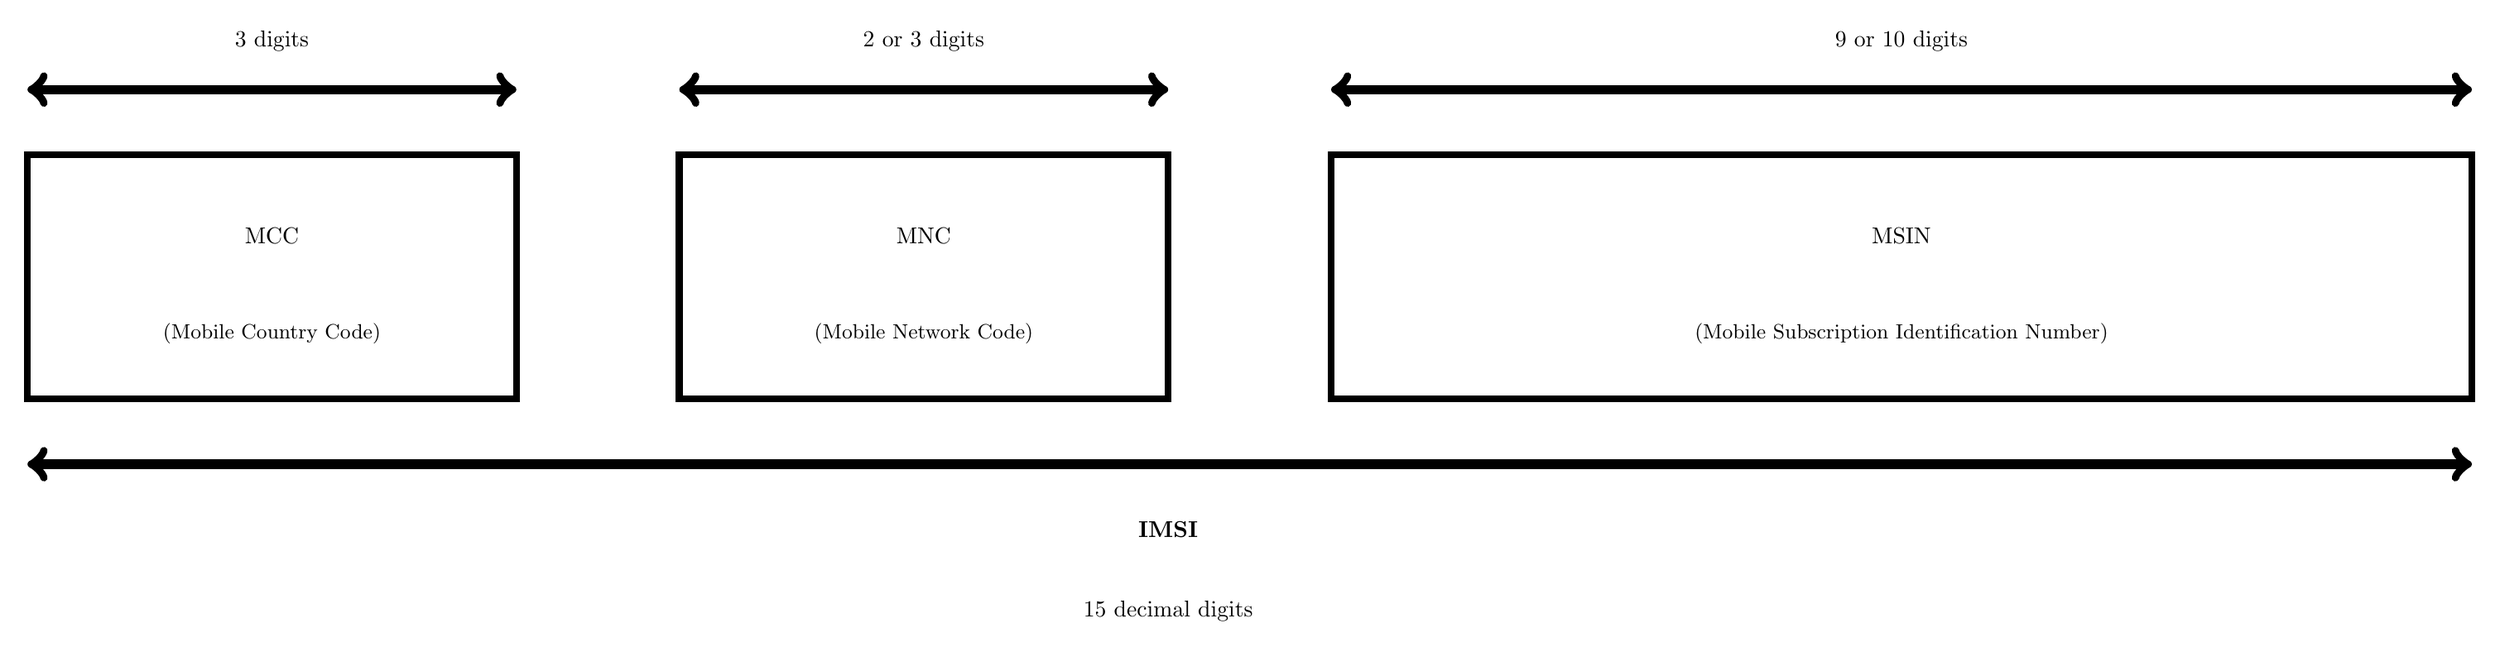
\begin{tikzpicture}[scale=5]



\filldraw[draw=black,fill=white,line width = 3pt] (0,0) rectangle (1.5,.75);
\draw [black, line width = 4pt, <->] (0,.95) -- (1.5,.95);
\draw node at (.75,1.1) {3 digits};
\draw node at (.75,.5) {MCC};
\draw node at (.75,.2) {\small (Mobile Country Code)};

\filldraw[draw=black,fill=white,line width = 3pt] (2,0) rectangle (3.5,.75);
\draw [black, line width = 4pt, <->] (2,0.95) -- (3.5,0.95);
\draw node at (2.75,1.1) {2 or 3 digits};
\draw node at (2.75,.5) {MNC};
\draw node at (2.75,.2) {\small (Mobile Network Code)};

\filldraw[draw=black,fill=white,line width = 3pt] (4,0) rectangle (7.5,.75);
\draw [black, line width = 4pt, <->] (4,0.95) -- (7.5,0.95);
\draw node at (5.75,1.1) {9 or 10 digits};
\draw node at (5.75,.5) {MSIN};
\draw node at (5.75,.2) {\small (Mobile Subscription Identification Number)};

\draw node at (3.5,-.4) {\textbf{IMSI}};
\draw node at (3.5,-.65) {15 decimal digits};


\draw [black, line width = 4pt, <->] (0,-0.2) -- (7.5,-0.2);

\end{tikzpicture}


\end{center}


\section{Mobile Network}
The SN and the HN are in a roaming contract. In case the UE is not roaming, SN and HN are the same network.

\begin{center}
    \begin{tikzpicture}[scale=2.7]



\node[inner sep=0pt] (wsn) at (-0.1,12) {\includegraphics[height = 3cm]{smartphone.png}};
\draw node at (-0.1,11.2) {\textbf{UE}};
\draw node at (-0.1,10.8) { (User Equipment)};

\node[inner sep=0pt] (wsn) at (6,12) {\includegraphics[height = 3cm]{tower.jpg}};
\filldraw[draw=white,fill=white] (5.5,11.4) rectangle (6.5,11.6);
\draw node at (6,11.2) {\textbf{SN}};
\draw node at (6,10.8) { (Serving Network)};

\node[inner sep=0pt] (wsn) at (11,12) {\includegraphics[height = 3cm]{home_network.jpg}};
\draw node at (11,11.2) {\textbf{HN}};
\draw node at (11,10.8) { (Home Network)};
%\draw node at (12,10.6) {\small The user is subscribed with};



\draw [black, line width = 4pt] (-0.15,10.3) -- (-0.15,7.5);

\draw [black, line width = 4pt] (6,10.3) -- (6,7.5);

\draw [black, line width = 4pt] (11,10.3) -- (11,7.5);


%\node[draw, double arrow, minimum height=120mm, minimum width=20mm, single arrow head extend=2mm, anchor=center, line width = 2pt] at (9,12) {};
%\draw node at (9,12) {\small Roaming agreement};


\draw [black, line width = 4pt, ->] (6.0,9) -- (-0.15,9);
\draw node at (3,10.2) {Want to use the service?};
\draw node at (3,9.8) {Reveal \textbf{IMSI}};
\draw node at (3,9.4) {so that you can be billed.};


\draw [black, line width = 4pt, ->] (-0.15,8) -- (6,8);
\draw node at (3,8.4) {\textbf{IMSI}};

\end{tikzpicture}


\end{center}

%\section{Passive IMSI Catchers}


%A passive IMSI catcher is always listening and waiting for an IMSI to be sent in plaintext.

%\begin{center}
%    \begin{tikzpicture}[scale=2.75]


\node[inner sep=0pt] (wsn) at (12,12)
    {\includegraphics[height = 3cm]{home_network.jpg}};
\draw node at (12,11.2) {\textbf{HN}};

\draw [black, line width = 4pt] (12,11) -- (12,7.5);

\node[inner sep=0pt] (wsn) at (6,12)
    {\includegraphics[height = 3cm]{tower.jpg}};
\filldraw[draw=white,fill=white] (4.5,11.25) rectangle (6.5,11.6);

\draw node at (6,11.2) {\textbf{SN}};

\draw [black, line width = 4pt] (6,11) -- (6,7.5);



\node[inner sep=0pt] (wsn) at (0,11.9)
    {\includegraphics[height = 3cm]{smartphone.png}};
\draw node at (0,11.2) {\textbf{UE}};


\draw [black, line width = 4pt] (0,11) -- (0,7.5);


\draw [black, line width = 4pt, ->] (6.0,10) -- (0,10);
\draw node at (3.0,10.5) {\small Want to use the service?};
\draw node at (3.0,10.2) {\small Reveal your \textbf{IMSI} so that you can be billed.};


\draw [black, line width = 4pt, <-] (6,9) -- (0,9);
\draw node at (3,9.2) {\small \textbf{IMSI}};

\node[inner sep=0pt] (wsn) at (3,12)
    {\includegraphics[height = 3cm]{listening_tower.png}};
\draw [red, dotted, line width = 1pt] (3,10.75) -- (3,8);
\draw node at (3,11.2) {\small \textbf{\textcolor{red}{Passive IMSI Catcher}}};
\draw node at (3,10.9) {\small \textbf{\textcolor{red}{Evesdropping only}}};

\filldraw[-, dotted, fill opacity=0.1, cyan,line width = 3pt] (3,12.3) arc (90:450:2.5);


\end{tikzpicture}


%\end{center}

%Protected in GSM, 3G and LTE. It will be protected in 5G too.
                                                                                                                                                                     


\section{Active IMSI Catchers}

An active IMSI catcher impersonates a legitimate SN.


\begin{center}
    \input{active_imsi_catcher.tikz}
\end{center}

\begin{Large}
No protection in GSM, 3G and LTE. There will be a protection in 5G.  
\end{Large}




\section{Defeating IMSI Catchers in 5G (Standardized)}
3GPP has decided to solve the problem using public-key encryption as follows.

\begin{center}
    \begin{tikzpicture}[scale=2.75]


\node[inner sep=0pt] (wsn) at (12,12)
    {\includegraphics[height = 3cm]{home_network.jpg}};
\draw node at (12,11.2) {\textbf{HN(5G)}};

\draw node at (10.6,13.5) { HN's public key: $\mathit{pk}$};
\draw node at (10.7,13) {HN's private Key: $\mathit{sk}$};

\draw [black, line width = 4pt] (12,11) -- (12,7.75);

\node[inner sep=0pt] (wsn) at (6,12)
    {\includegraphics[height = 3cm]{tower.jpg}};
\filldraw[draw=white,fill=white] (4.5,11.25) rectangle (6.5,11.6);

\draw node at (6,11.2) {\textbf{SN(5G)}};

\draw [black, line width = 4pt] (6,11) -- (6,7.75);



\node[inner sep=0pt] (wsn) at (0,11.9)
    {\includegraphics[height = 3cm]{smartphone.png}};
\draw node at (0,11.2) {\textbf{UE(5G)}};

\draw node at (1.6,13) {HN's public key: $\mathit{pk}$};


\draw [black, line width = 4pt] (0,11) -- (0,7.75);


\draw [black, line width = 4pt, ->] (6.0,10) -- (0,10);
\draw node at (3.0,10.4) {Reveal \textbf{IMSI}};


\draw [black, line width = 4pt, <-] (6,9) -- (0,9);
\draw node at (3,9.4) {$\text{MCC},\text{MNC},E_{\mathit{pk}}(\text{MSIN})$};

\draw [black, line width = 4pt, ->] (6,9) -- (12,9);
\draw node at (9,9.4) { $E_{\mathit{pk}}(\text{MSIN})$};

\draw [black, line width = 4pt, <-] (6,8) -- (12,8);
\draw node at (9,8.4) {MSIN};


\end{tikzpicture}


\end{center}



\section{Downgrade Attack}

\begin{Large}
5G and LTE interworks $\Rightarrow$ An LTE based active IMSI catcher can mount an attack. 
\end{Large}



\begin{center}
    \begin{tikzpicture}[scale=2.75]


\node[inner sep=0pt] (wsn) at (12,12)
    {\includegraphics[height = 3cm]{home_network.jpg}};
\draw node at (12,11.2) {\textbf{HN (5G)}};

\draw [black, line width = 4pt] (12,11) -- (12,6.8);

\node[inner sep=0pt] (wsn) at (6,12)
    {\includegraphics[height = 3cm]{tower.jpg}};
\filldraw[draw=white,fill=white] (4.5,11.25) rectangle (6.5,11.6);

\draw node at (6,11.2) {\textbf{SN(LTE/5G)}};

\draw [black, line width = 4pt] (6,11) -- (6,6.8);

\node[inner sep=0pt] (wsn) at (0,11.9)
    {\includegraphics[height = 3cm]{smartphone.png}};
\draw node at (0,11.2) {\textbf{UE}};

\draw [black, line width = 4pt] (0,11) -- (0,6.8);


\draw [black, line width = 3pt, <->] (6.0,10) -- (0,10);
\draw node at (3.0,10.2) {\small Established connection};


\draw [black, line width = 4pt, ->] (3,9) -- (0,9);
\draw node at (1.5,9.5) {\small Stronger Signal};
\draw node at (1.5,9.2) {\small Reveal \textbf{IMSI}};

\draw [black, line width = 3pt, <->] (6.0,8) -- (0,8);
\draw node at (1.5,8) {\Huge \textcolor{red}{$\times$}};

\draw [black, line width = 4pt, <-] (3,7) -- (0,7);
\draw node at (1.5,7.2) {\small \textbf{IMSI}};


\node[inner sep=0pt] (wsn) at (3,12)
    {\includegraphics[height = 3cm]{listening_tower.png}};
\draw [red, line width = 2pt,dotted,] (3,10.7) -- (3,6.8);
\draw node at (3,11.2) {\small \textbf{\textcolor{red}{Fake SN (LTE)}}};
\draw node at (3,10.9) {\small \textbf{\textcolor{red}{Active IMSI Catcher}}};

%\filldraw[-, dotted, fill opacity=0.2, cyan,line width = 3pt] (3,12.3) arc (90:450:2.5);


\end{tikzpicture}


\end{center}


\section{Defeating Downgrade Attack}


 \begin{Large}
 Hybrid solution using public-key encryption and pseudonyms. 
 \end{Large}
 
 %\cite{Norrman_Naslund_Dubrova_2016,Ginzboorg_Niemi_2016,CCS15,SSR15}. 
 

\vspace{.5cm}
{\Large\usefont{T1}{phv}{bx}{n}\textcolor{facultyColor}{\MakeUppercase{5G SN:}} \MakeUppercase{}}\\

\begin{center}
    \input{defeating_downgrade_attack.tikz}
\end{center}

\vspace{.5cm}
{\Large\usefont{T1}{phv}{bx}{n}\textcolor{facultyColor}{\MakeUppercase{LTE SN:}} \MakeUppercase{}}\\


\begin{center}
    \input{defeating_downgrade_attack_LTE.tikz}
\end{center}

\subsection*{Advantages}
%\begin{large}
\begin{itemize}
 \item No standardization. Works even when $\text{EAP-AKA}^{'}$ is used.
 \item Major Disadvantages of pseudonym based solution disappears 
  \begin{itemize}
   \item In case of de-synchronization of pseudonyms, resynchronization can be done just by connecting through a 5G SN.
   \item A malicious SN can not mount an attack to de-synchronize pseudonyms, because the HN verifies the success of a 5G AKA and $\text{EAP-AKA}^{'}$.
   \item Hence, the management of pseudonyms in the subscriber database becomes less vulnerable to unwanted modification.
  \end{itemize}
\end{itemize}
%\end{large}

\subsection*{Challenges}
%\begin{large}
\begin{itemize}
 \item A 5G UE may connect with multiple SNs. Thus the UE will have multiple active connection using different pseudonyms simultaneously. These may create complications -- when a UE or the HN may forget an old pseudonym.
 \item SN has to rely on the HN for lawful interception -- identifying a user using SUPI (IMSI). 
\end{itemize}
%\end{large}

%\normalsize

%\bibliographystyle{plain}
%\bibliography{ref}

\end{multicols}

\vfill % some more marginal in the end

\begin{minipage}[t]{0.9\linewidth} % footer
\footnotesize
%\color{gray}{\textsf{\textbf{The {\LaTeX} template by Jussi Tiira used in this poster is licensed under a Creative Commons Attribution 4.0 International License.}}}
\end{minipage}


\end{document}
